\documentclass[]{scrartcl}
\usepackage{graphicx}
\usepackage[dvipsnames]{xcolor}
\definecolor{mygray}{gray}{0.9}

% Title Page
\title{\textbf{Parallel computing - Exercise 2}}
\author{Michela Venturini}
\date{Spring 2019}

\begin{document}
\maketitle

\section{Parallelize code by using OpenMP}

The task of the exercise consists in paralelizing a given chunk of code to visualize OpenMP scheduling of the threads. The scheduling of the \textit{for loop} of the code is specified by the option \colorbox{mygray}{\texttt{\#pragma omp for schedule([type\_of\_scheduling]) private(i)}}. The scheduling can be static or dynamic and it is also possible to specify the size of the chunk being assigned to each thread.
\begin{itemize}
\item[\textbf{static}] The static option impiles that iterations blocks are mapped statically to the execution threads in a round-robin fashion. 
\item[\textbf{dynamic}] The dynamic sheduling works on first-come first-served policy. This implies that different executions of the same code with the same number of threads may produce different results. This strategy can lead a better workload balancing w.r.t. the previuous one but might introduce some additional overhead.
\end{itemize}

\section{Execution}
The code is executed on Ulysses by using the options:
\begin{enumerate}
	\item static
	\item static, with chunk size 1
	\item static, with chunk size 10
	\item dynamic
	\item dynamic, with chunk size 1
	\item dynamic, with chunk size 10
\end{enumerate}
The execution is performed by submitting a job on Ulysses through the command	\colorbox{mygray}{\texttt{qsub nodes=1:ppn=20 ex2.sh}} that asks for a single node, sufficient for this purpose.

\section{Results}
 The result of executions are presented in the \ref{fig_1}.
 As expected, the behaiviour of \texttt{dynamic} executions leads to a different result in the scheduling of the threads that is not fixed as in the other case. 
 \begin{figure}[h!]
 	\begin{centering}
 		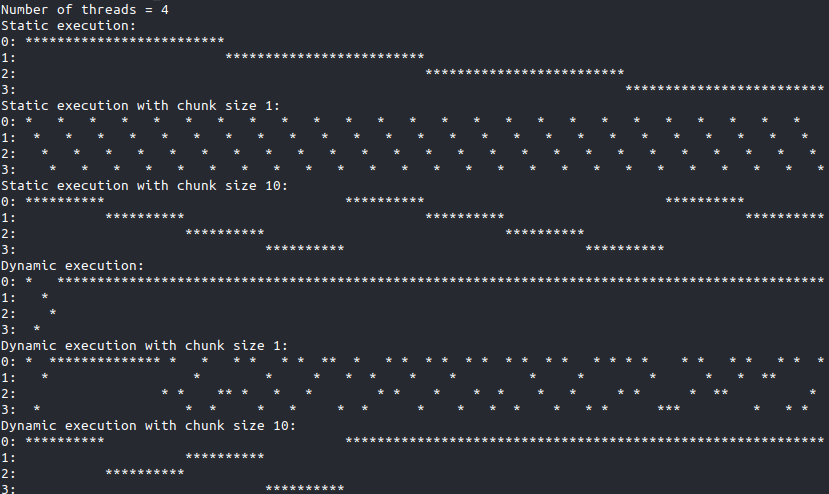
\includegraphics[scale=.5]{img_ex2}
 		\caption{Result of the executions with 4 threads}
 		\label{fig_1}
 	\end{centering}
 \end{figure} 
\end{document} 